\documentclass[12pt]{article}
\usepackage{fancyhdr}
\usepackage{datetime}
\usepackage{enumitem}
\usepackage{float}
\usepackage{graphicx}
\usepackage{amsmath}
\graphicspath{ {images/} }
%\usepackage{showframe}

%custom variables
\newdate{date}{28}{10}{2016}
\newcommand{\hwNum}{2}
\newcommand{\assign}{Homework }
\newcommand{\class}{EC441: }
\newcommand{\name}{Daniel Andronov}


%header
\pagestyle{fancy}
\lhead{\name{}}
\chead{\thepage}
\rhead{\class{}\assign{}\hwNum{}}
\cfoot{\thepage}

\fancyheadoffset[LO,RE]{1pt}
\fancyheadoffset[RO,LE]{1pt}


%titlepage
\title{\class{}\assign{}\hwNum{}}
\author{\name{}}
\date{\displaydate{date}}


%addition settings
\topmargin=-0.45in
\evensidemargin=0in
\oddsidemargin=0in
\textwidth=6.5in
\textheight=9.0in
\headsep=0.25in

%adjusting vertical whitespace for the images at the top
\makeatletter
\setlength{\@fptop}{0pt}
\makeatother


%start the document
\begin{document}
\maketitle
\newpage

\section{Textbook Problems}
Problems from the book

\paragraph{Problem 2.23}
\begin{enumerate}[label=\textbf{Part \alph*)},leftmargin=*,align=left]
	\item if $t_{dist} = \frac{NF}{u_s}$, then the server's upload time dominates the client's slowest download time.
	\item if $t_{dist} = \frac{F}{d_{min}}$, then ther client's slowest download time dominates the upload time of the server.
	\item The minium distriubution time cannot be faster that the larger of the server's upload time or the slowed client download time, and thus $t_{dist} \geq max\{ \frac{NF}{ u_s}, \frac{F}{ d_{min}} \}$.
\end{enumerate}

\paragraph{Problem 3.3}
UDP takes the 1's complement sum so that checksum does not exceed 8 bits and can be easily checked for single bit errors. The computed checksum and the one that is computed on the receiver side should add up to all zero's using 1's complement addition, if there were no errors. Bit errors are detected by seeing which bits are set, and single bit errors can be corrected by seeing which single bit is set. However, this scheme is not fool-proof as is two bits are swapped in such a way that they still produce checksums that are complements of each other, the receiver can still compute the correct checksum and miss detecting the errors. \\
\begin{tabular}{ l | l | l | l | l | l | l | l | l | l |}
	    & 0&1&0&1&0&0&1&1 \\
	    & 0&1&1&0&0&1&1&0 \\
	+ & 0&1&1&1&0&1&0&0 \\
	\hline
	& 0&0&1&0&1&1&0&1\\
	+ &&&&&&&&1\\
	\hline
	&0&0&1&0&1&1&1&0\\
\end{tabular}
\\
Thus the 1's complement sum would be \texttt{00101110}.
\paragraph{Problem 3.13}
Say that the sender has already send out two packets and sends out two more,$p_0$ and $p_1$. If, while traveling through the network, $p_1$ arrives to the receiver before $p_0$, the receiver will think when it receive's $p_1$, that it is a duplicated packet and discard it when, in fact, it is a new packet entirely. 
	\begin{figure}[H]
		\caption{Space Time Diagram of reordered packets between two nodes using Stop \& Wait}
		\centering
		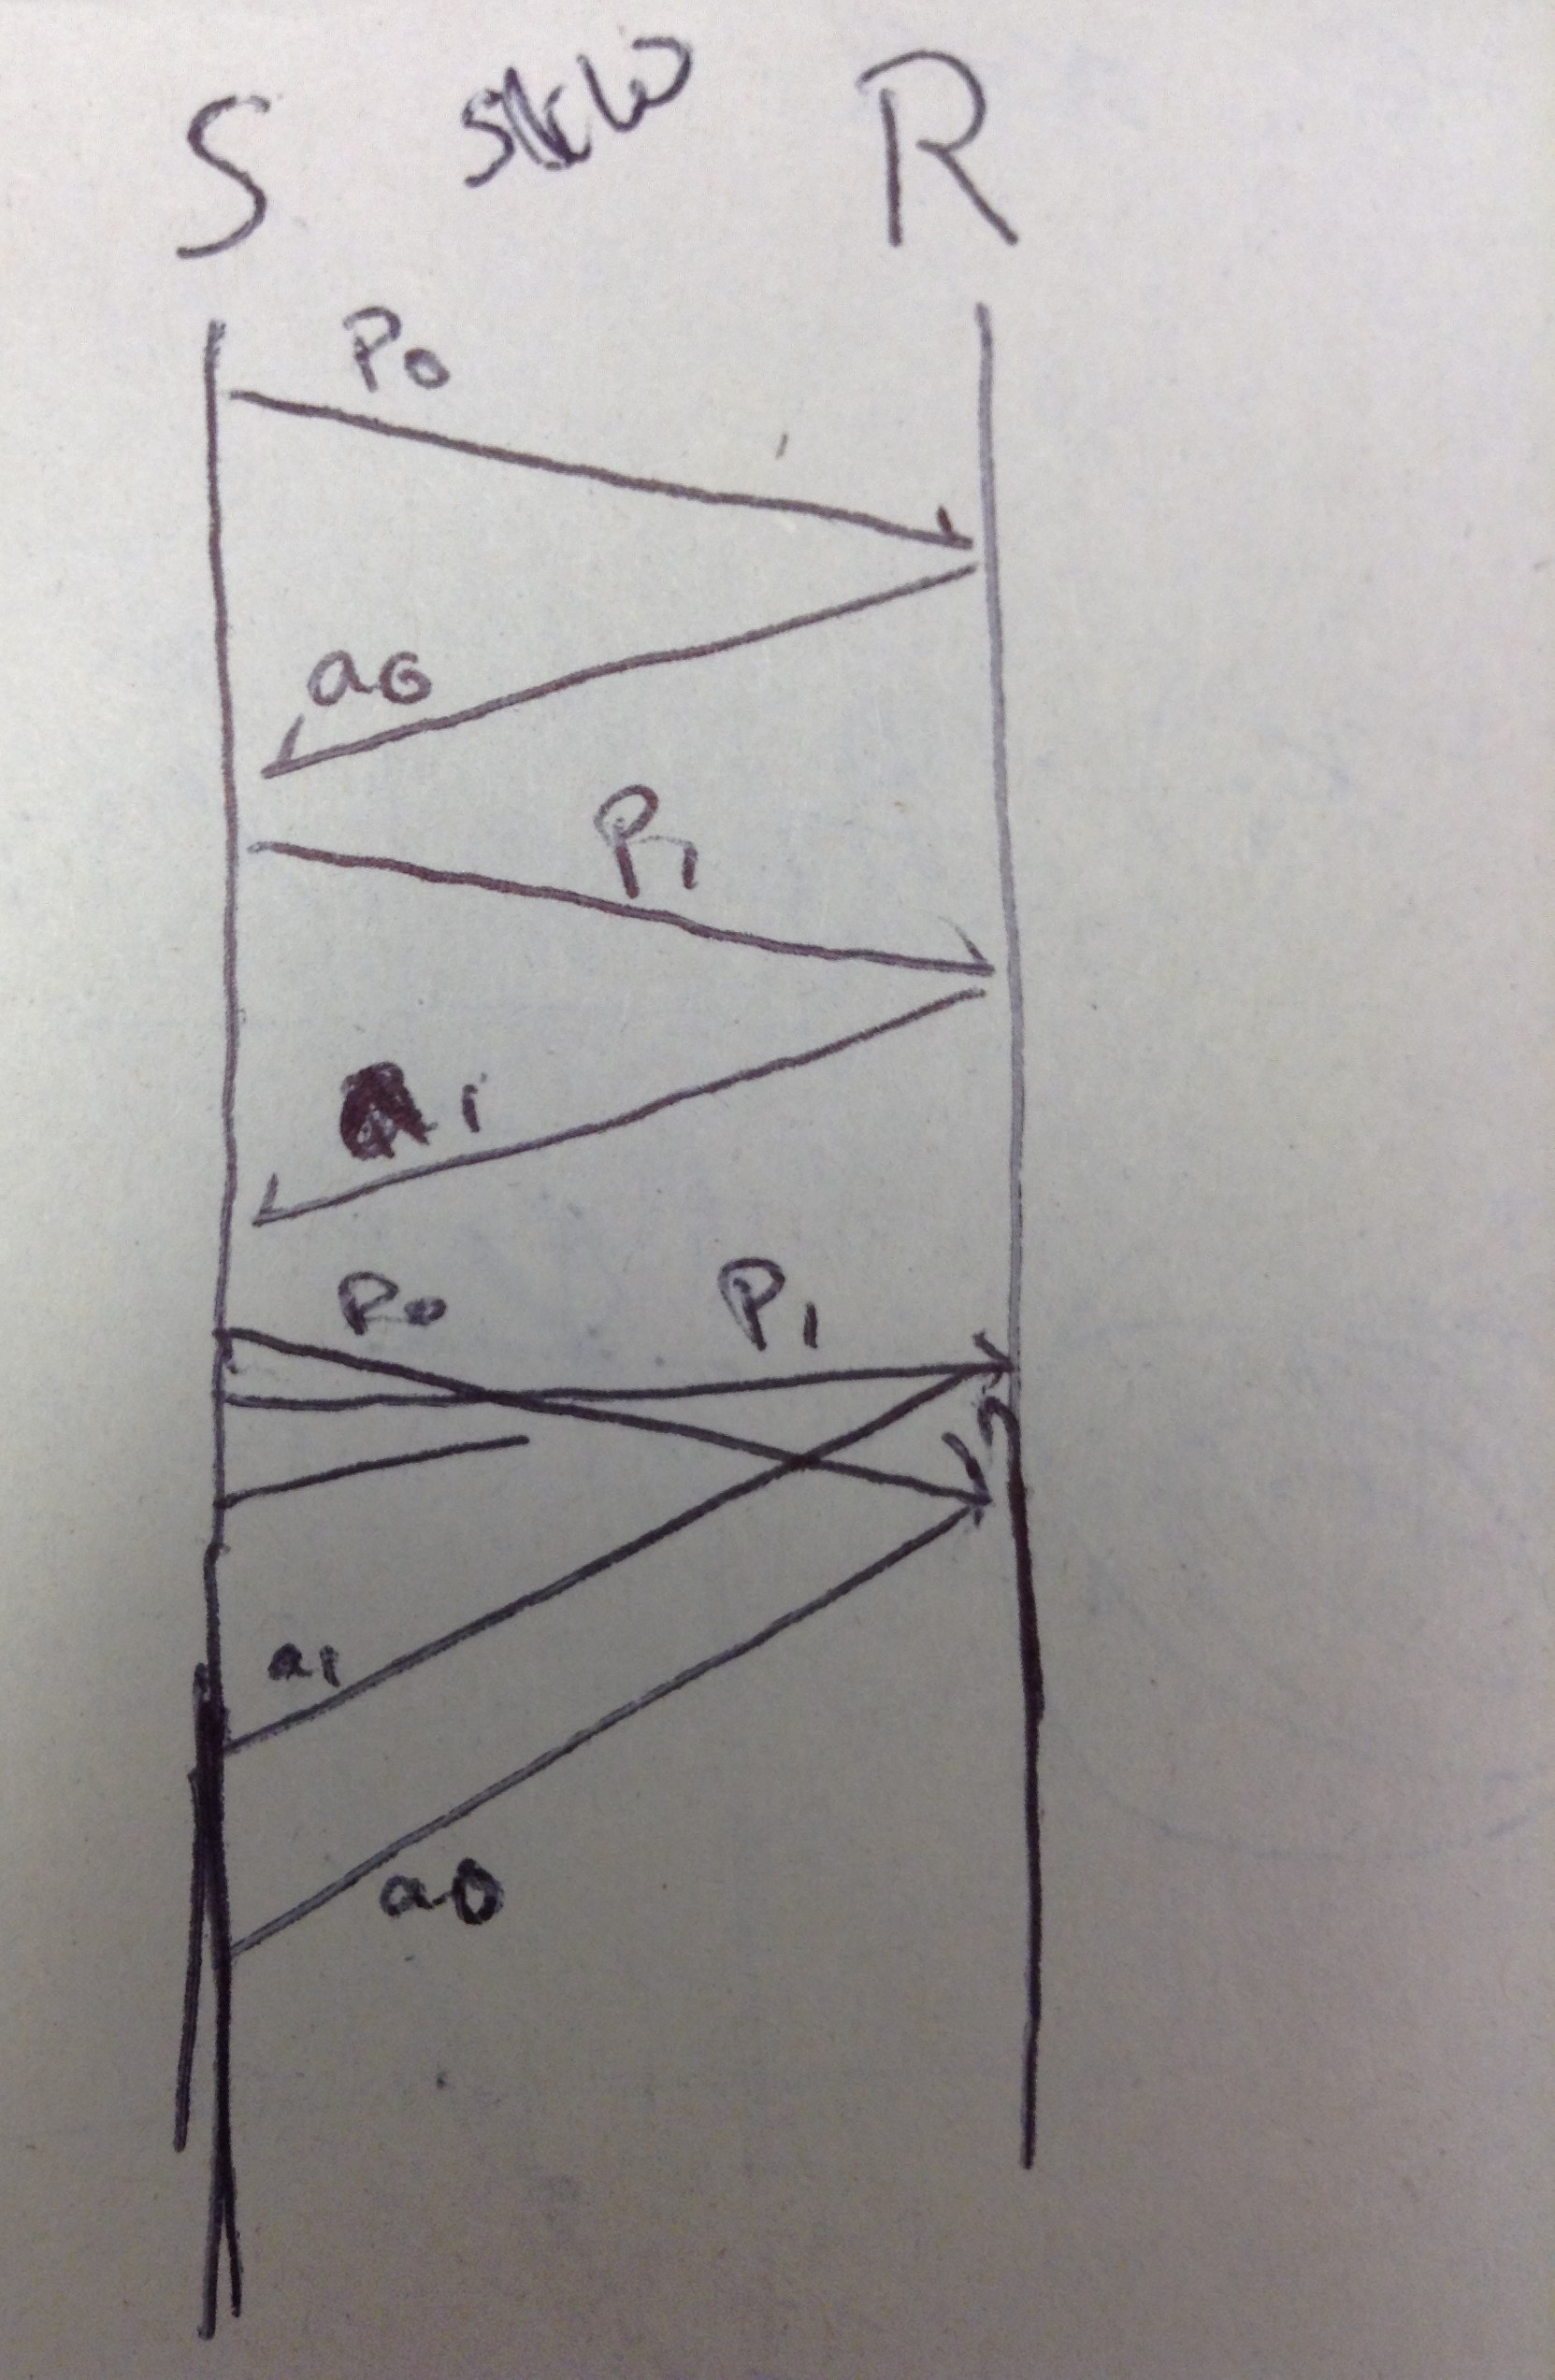
\includegraphics[scale=0.1]{SW_switch}	
	\end{figure}

\paragraph{Problem 3.19}
This protocol functions the same way as Stop \& Wait does except that now, acknowledgements need to specify which receiver they come from so that A know when to send the next packet to both B \& C.
\begin{figure}[H]
	\caption{FSM for A's protocol}
	\centering
	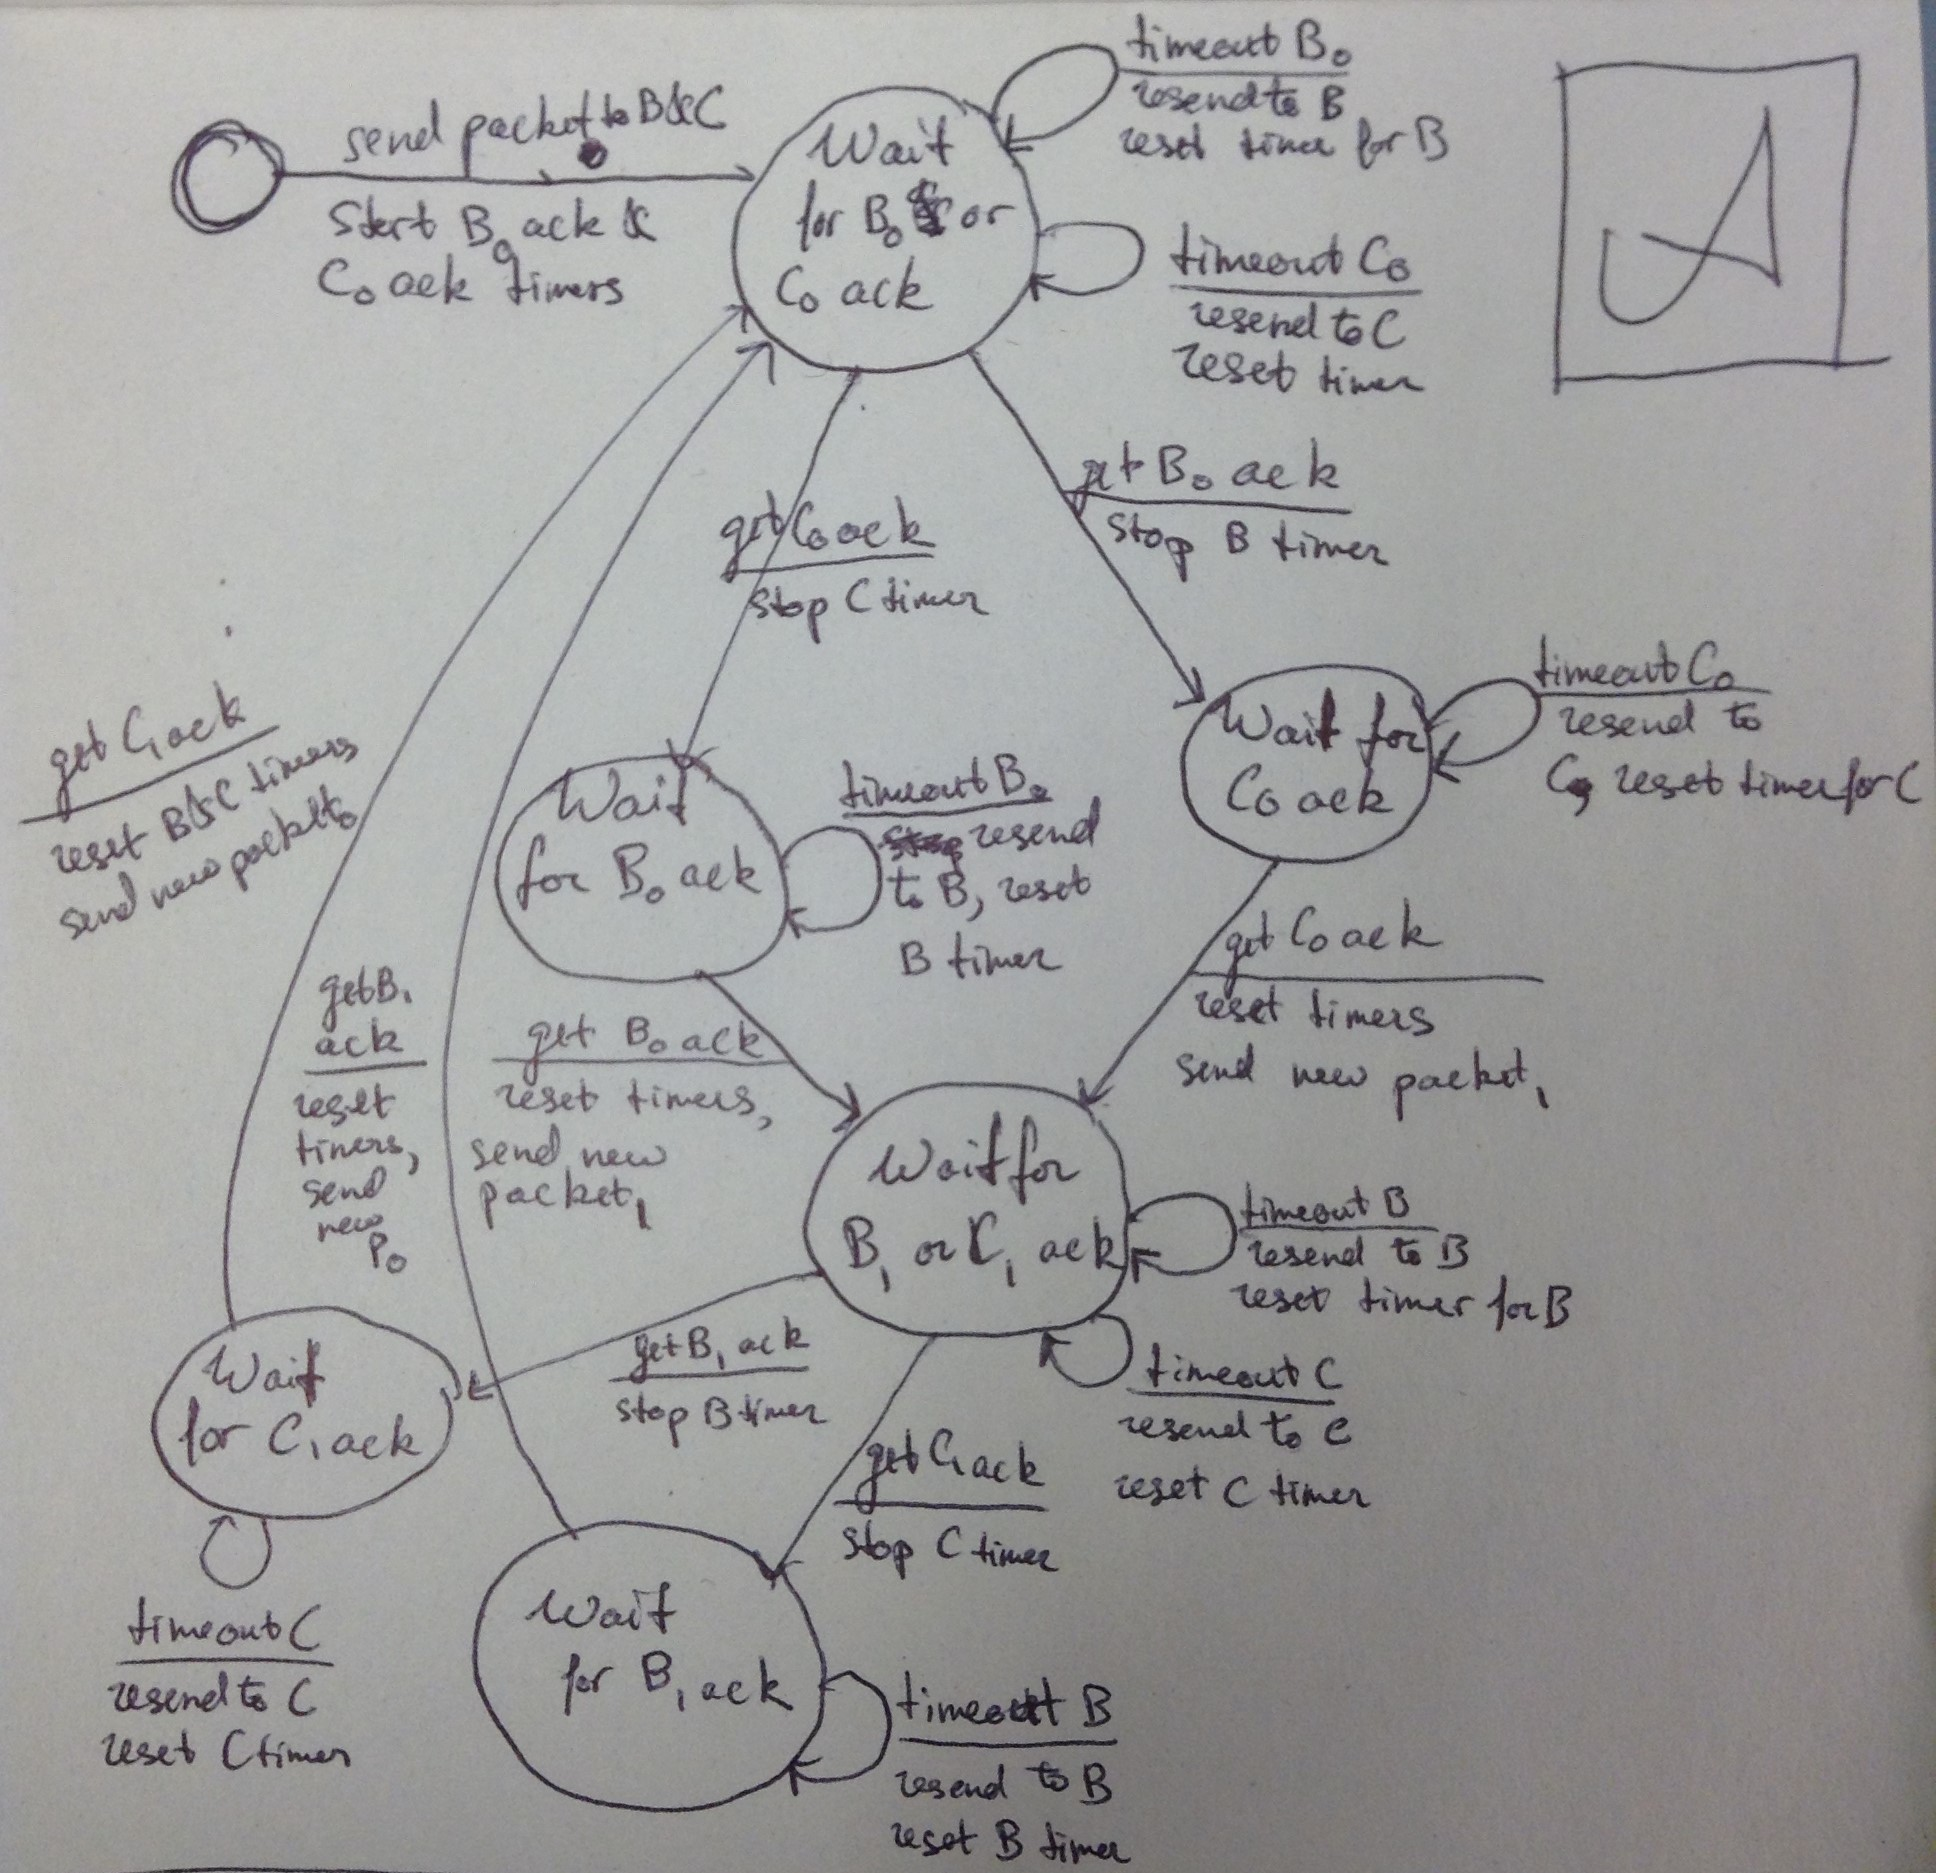
\includegraphics[width=\textwidth,scale=0.3]{A}	
\end{figure}
\begin{figure}[H]
	\caption{FSM of B \& C's protocol}
	\centering
	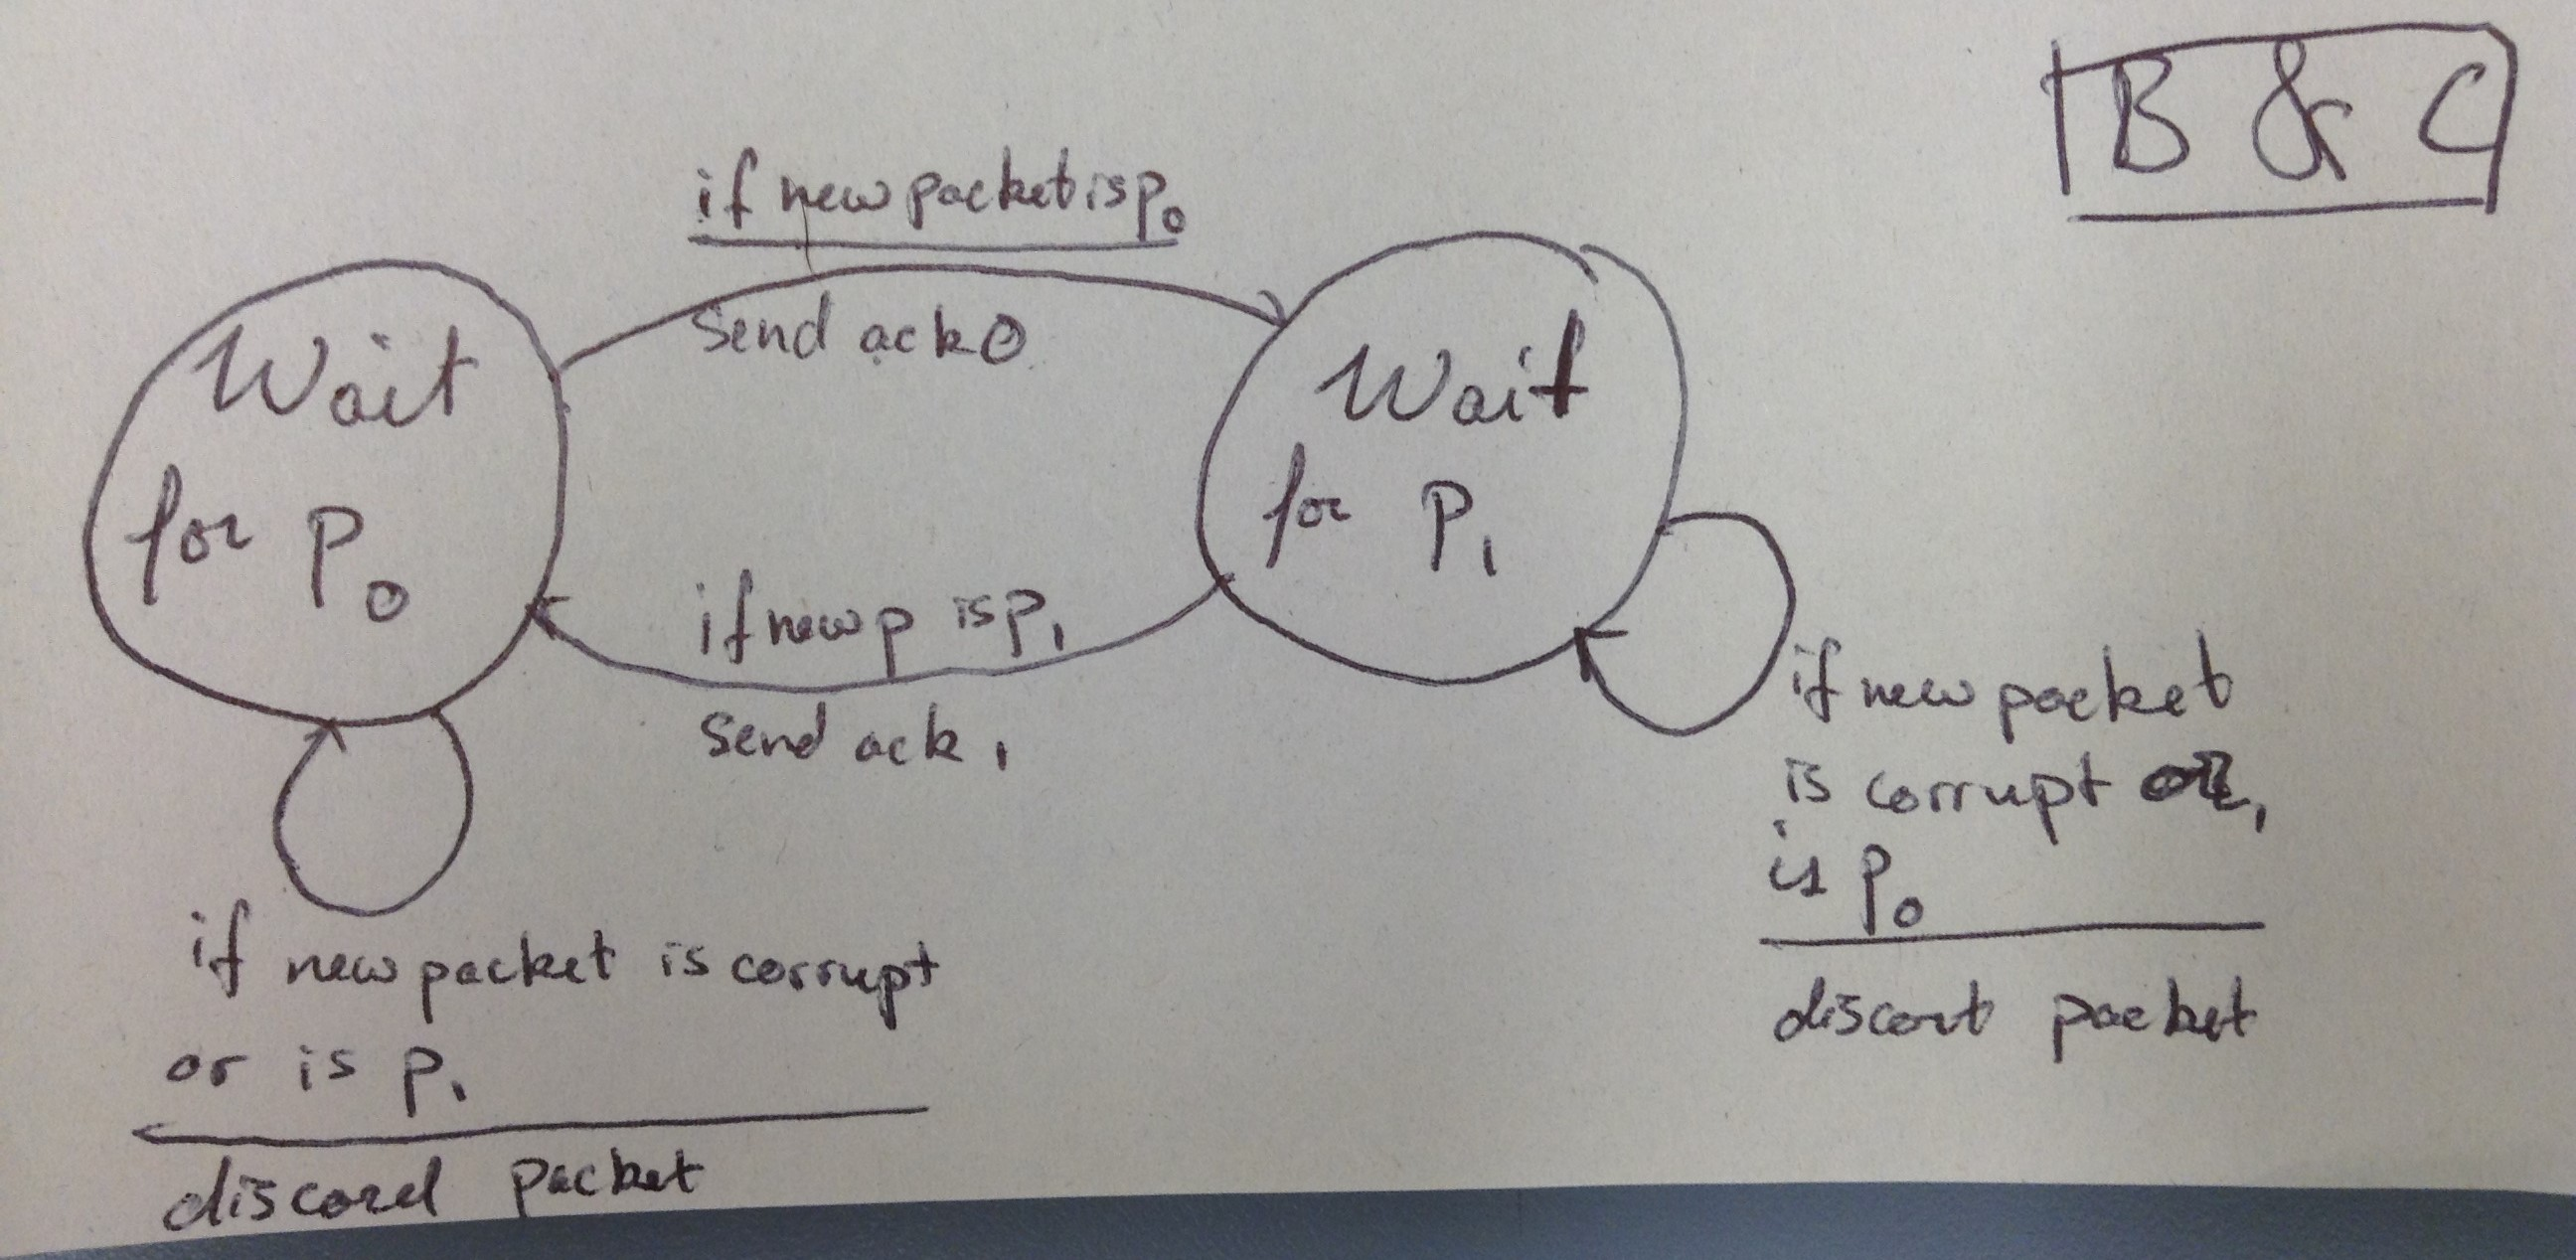
\includegraphics[width=\textwidth]{BC}	
\end{figure}

\paragraph{Problem 3.22}
\begin{enumerate}[label=\textbf{Part \alph*)},leftmargin=*,align=left]
	\item $k$ can be at either the front or the back of the window, e.g. $\{k-3, k-2, k-1, k\}$ or $\{k, k+1, k+2, k+3\}$, so the range should be $[k-3, k+3]$ or seven different numbers. 
	\item The maximum range of Ack values is equal to the sender's windwos size. This is because the receiver will only acknowledge the last received packet and does not acknowledge out of order packets. Thus, the receiver only needs to keep up with the packets in the sender's window.
\end{enumerate}

\paragraph{Problem 3.24}
\begin{enumerate}[label=\textbf{Part \alph*)},leftmargin=*,align=left]
	\item True, the window of the sender advances whenever the sender receives an acknowledgement. So if a time out is long enough, the sender window can receive other acknowledgements and advance the window past the packet that has not yet been acknowledged. 
	\item False, GBN will not advance a past a packet that has not been yet acknowledged. 
	\item False, SR will buffer out of order packets but the alternating bit protocol will discard packets that are out of order.
	\item True, GBN will discard out of order packets as the alternating bit protocol does.
\end{enumerate}
\section{Additional Questions}

\paragraph{Additional Question 1}
\begin{enumerate}[label=\textbf{Part \arabic*)},leftmargin=*,align=left]
	\item 
		\begin{enumerate}[label=\textbf{\alph*)}]
			\item Stop \& Wait : 1 bit.
			\item GBN, W = 4: 3 bits
			\item SR, W = 4: 4 bits;
		\end{enumerate}
	\item For all of the following parts, let $T$ be the time between the sender sending a packet and receving its corresponding acknowledgement packet.
		\begin{enumerate}[label=\textbf{\alph*)}]
			\item $t_{total} = 8T - t_{prop}$. $T = t_{xmit} + 2t_{prop} = 1ms + 2 \times 1ms = 3ms$. So, $t_{total} = 23ms$.
				\begin{figure}[H]
					\centering
					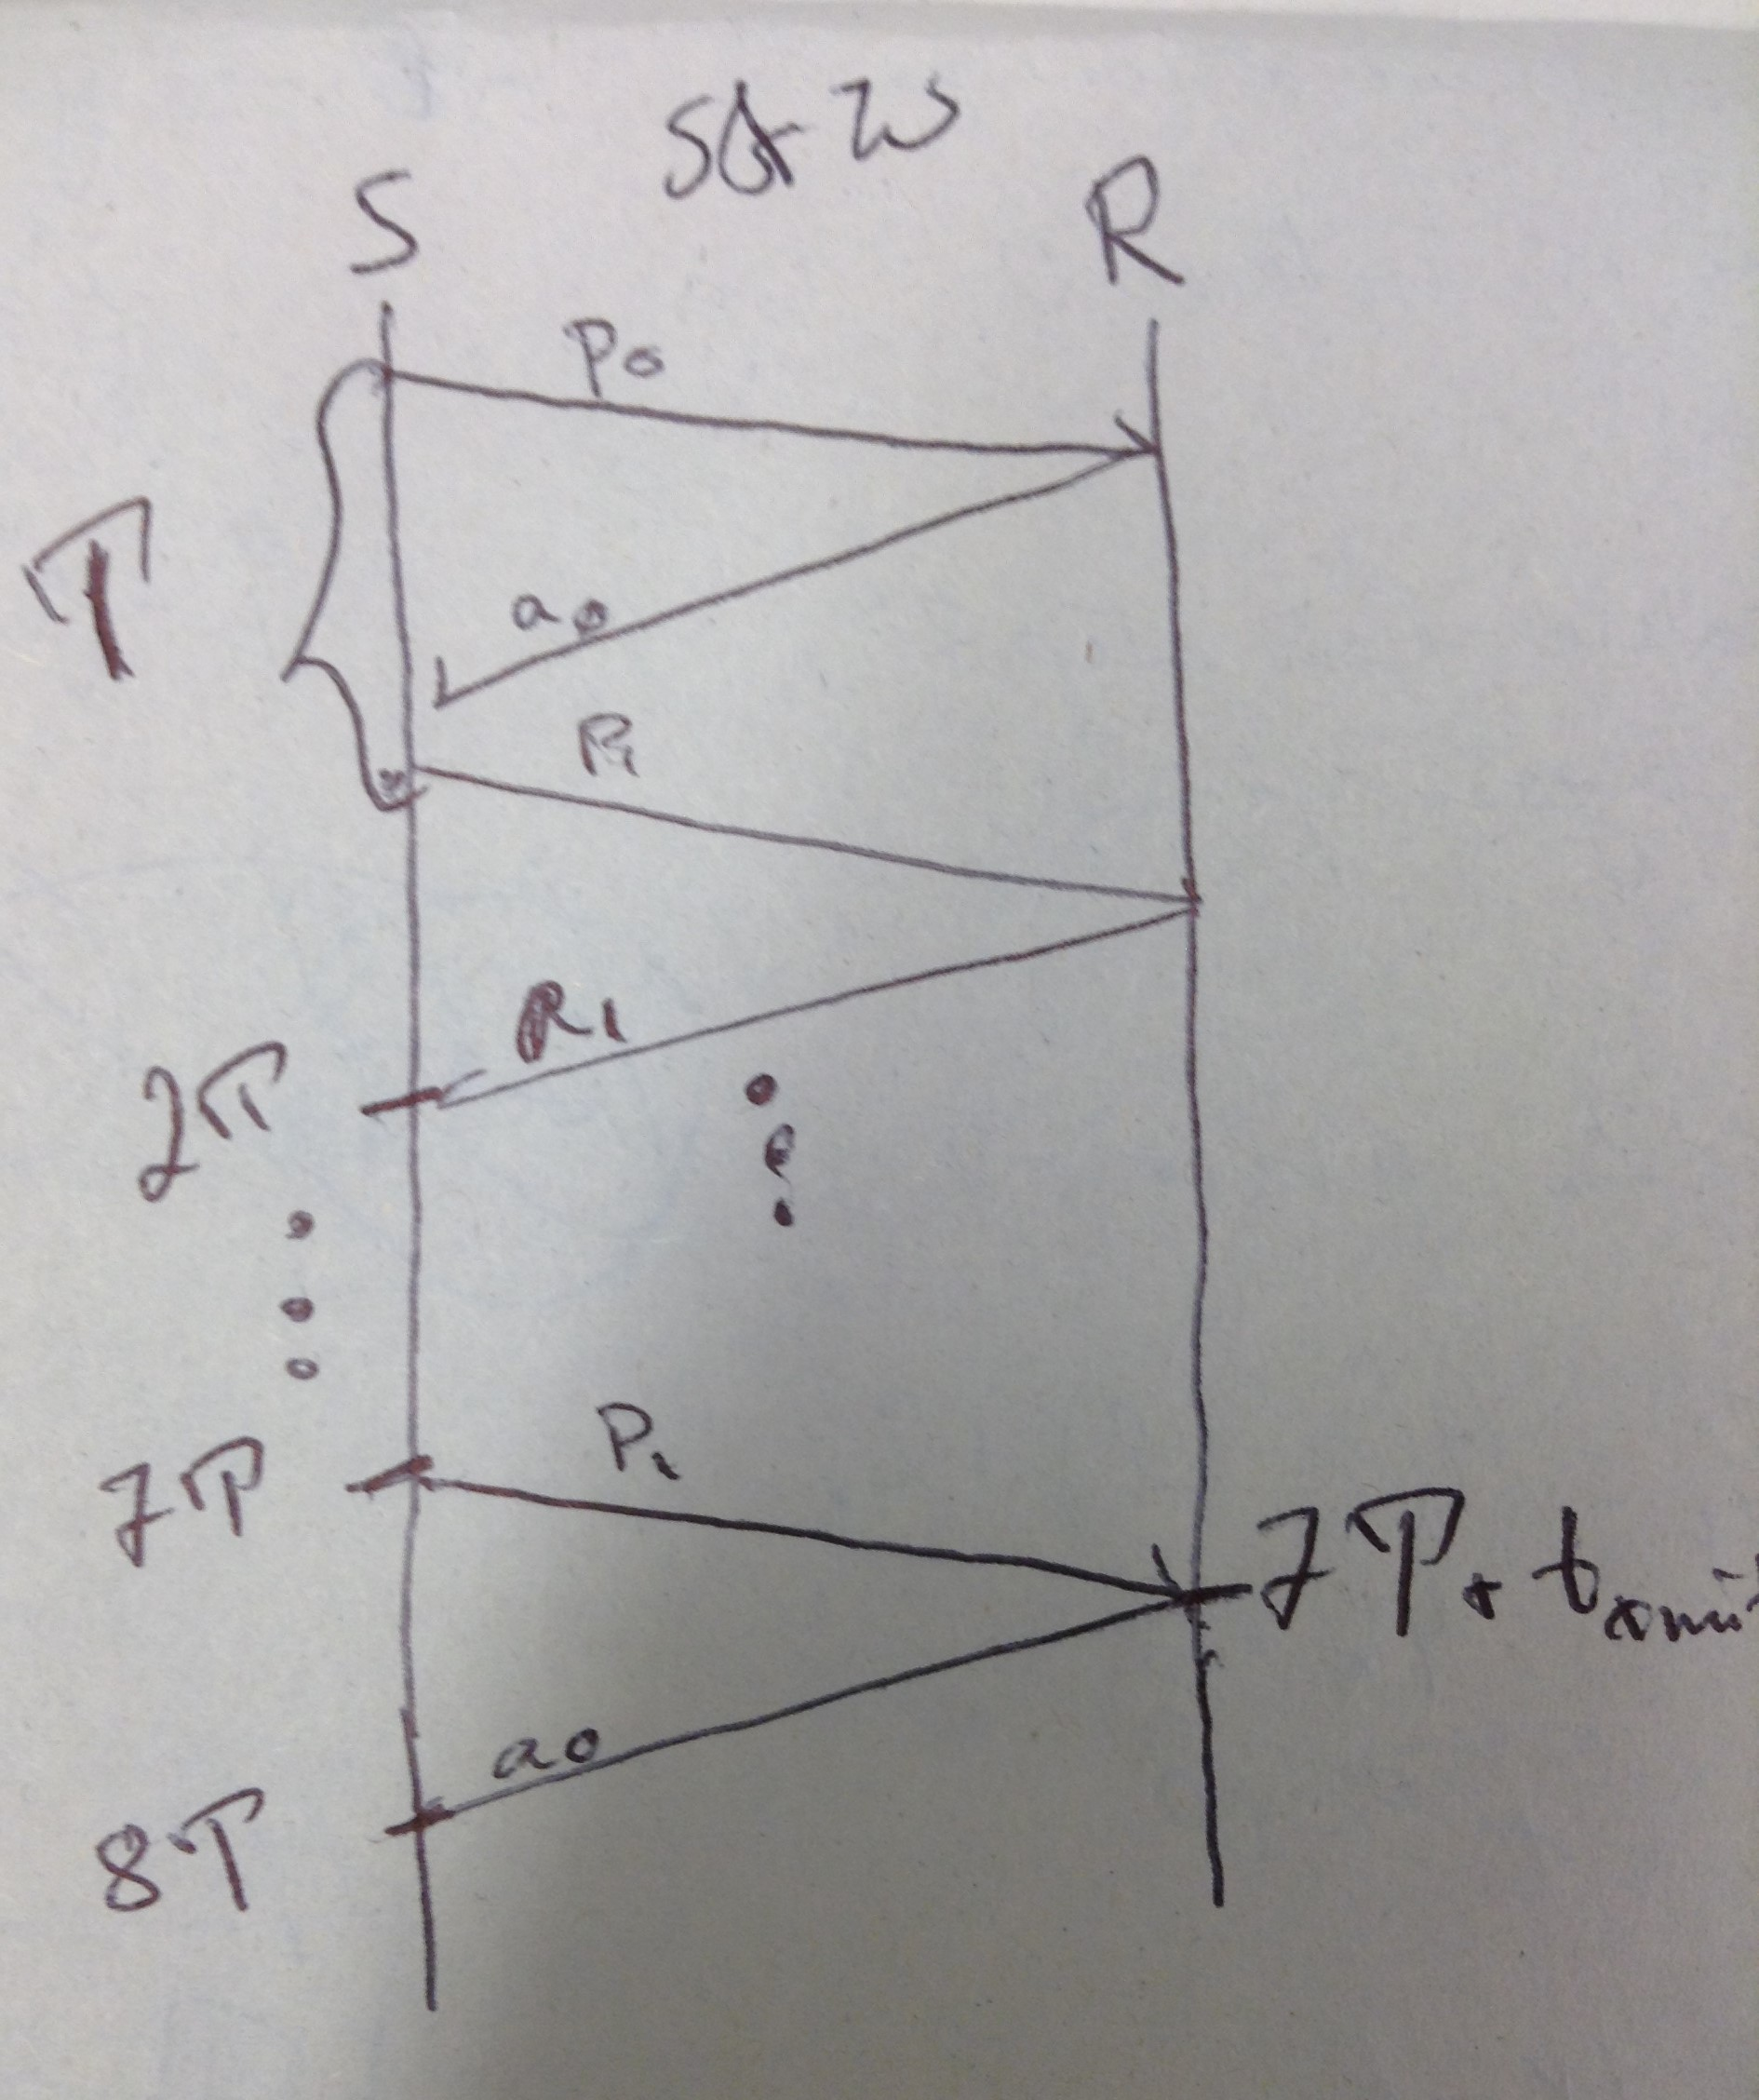
\includegraphics[scale=0.1]{SR8}	
				\end{figure}
			\item $t_{total} = 4t_{xmit} + T + t_{xmit} + t_{prop} = 4 \times 1ms + 3ms + 1ms + 1ms = 9 m$. So, $t_{total} = 9ms$.
				\begin{figure}[H]
					\centering
					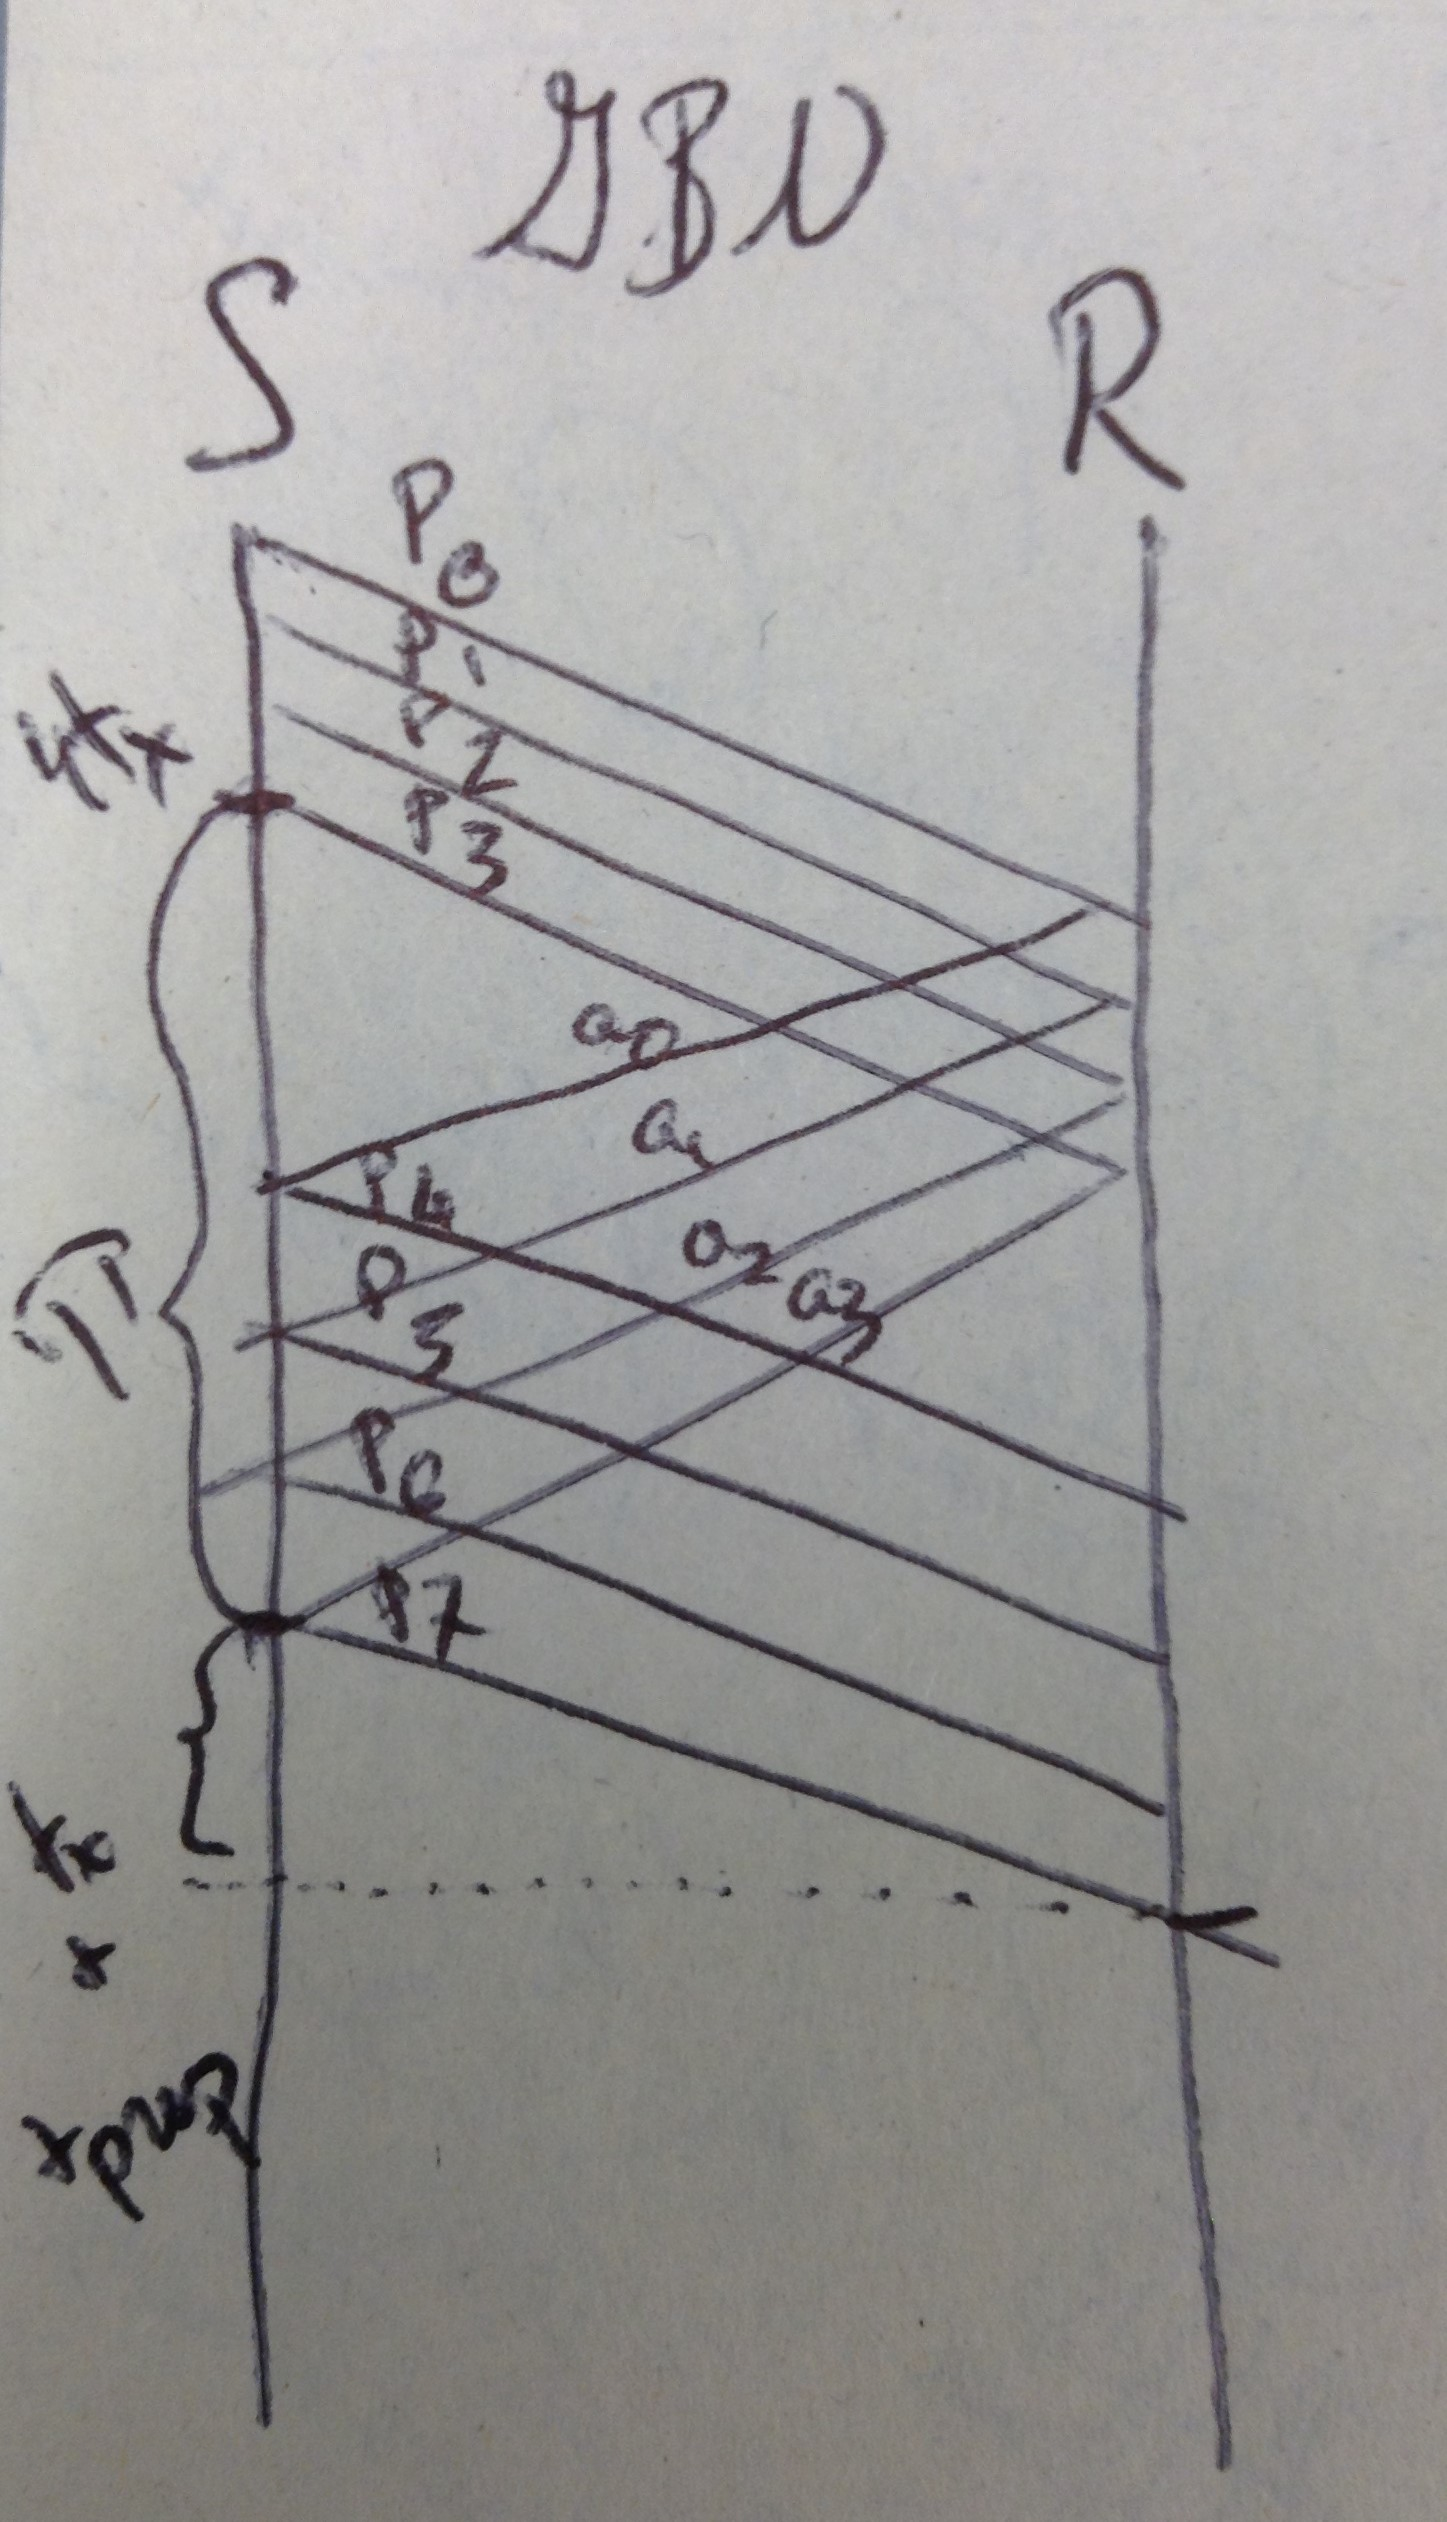
\includegraphics[scale=0.1]{GBN}	
				\end{figure}
			\item Same as GBM so, 9ms.
				\begin{figure}[H]
					\centering
					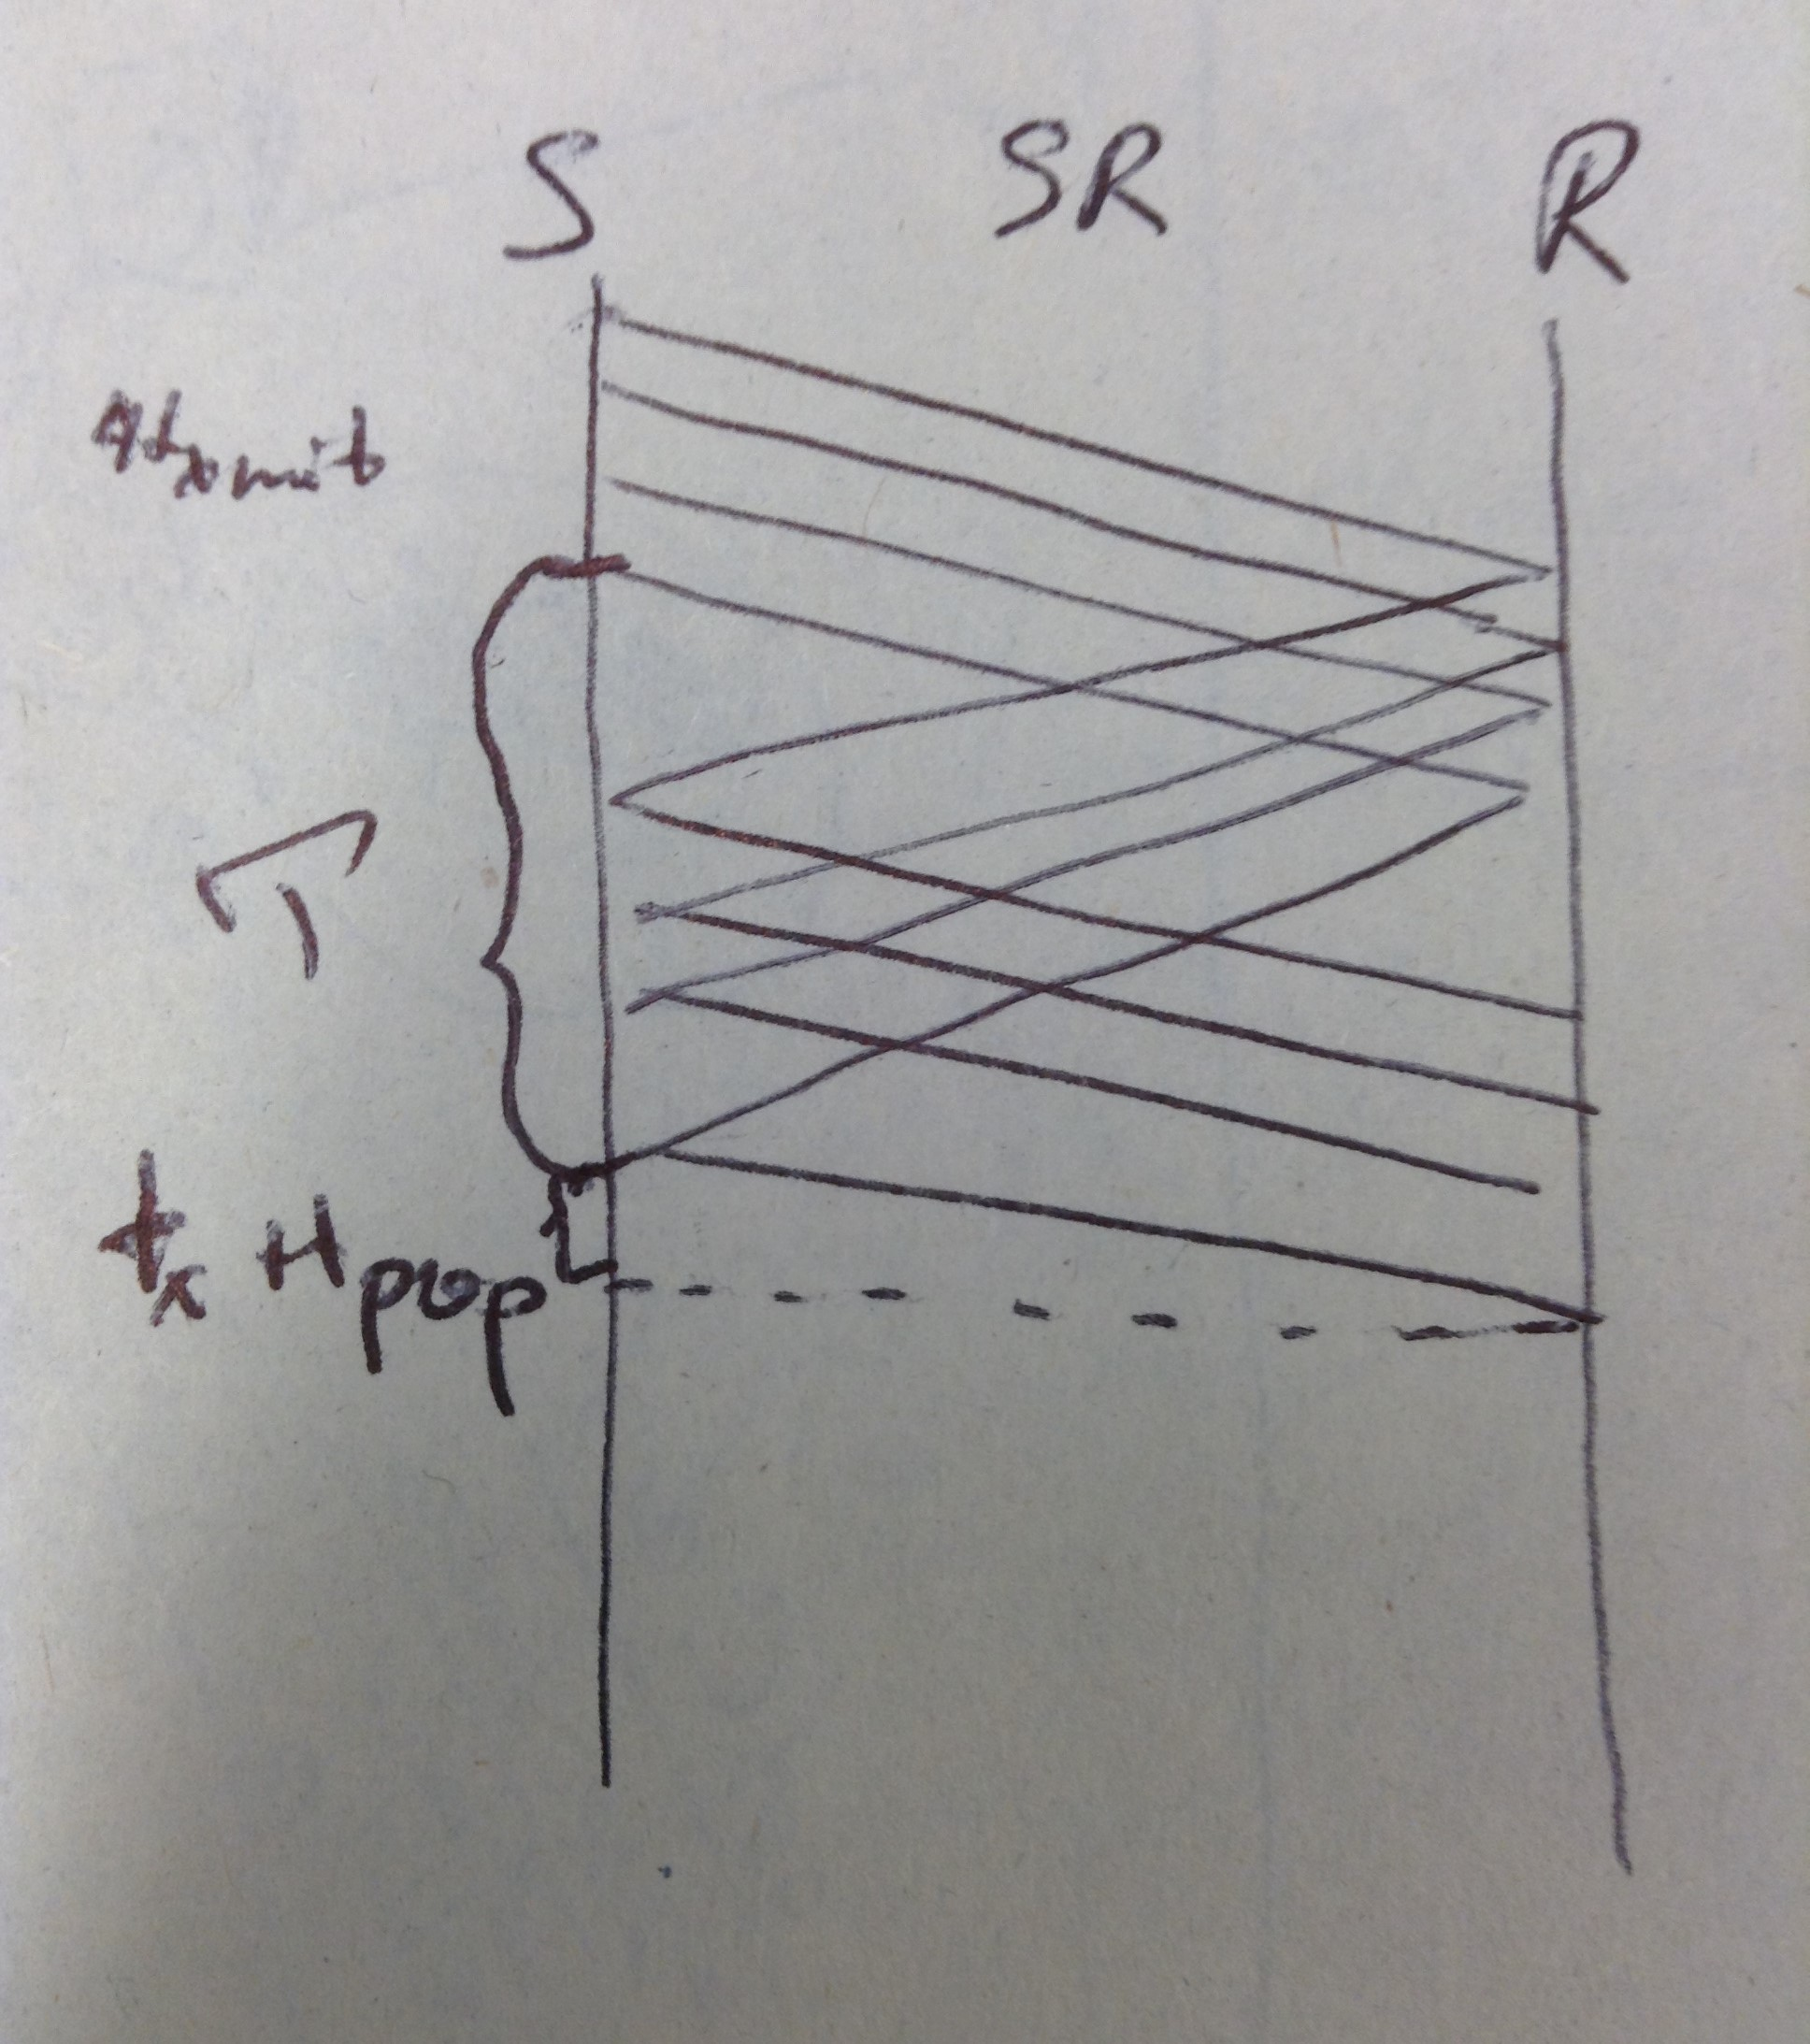
\includegraphics[scale=0.1]{SR}	
				\end{figure}
		\end{enumerate}
	\item
		\begin{enumerate}[label=\textbf{\alph*)}]
			\item For stop \& wait, the time will be the same as before except the sender will wait 5ms for the time out, so $t_{total} = 28ms$.\
				\begin{figure}[H]
					\centering
					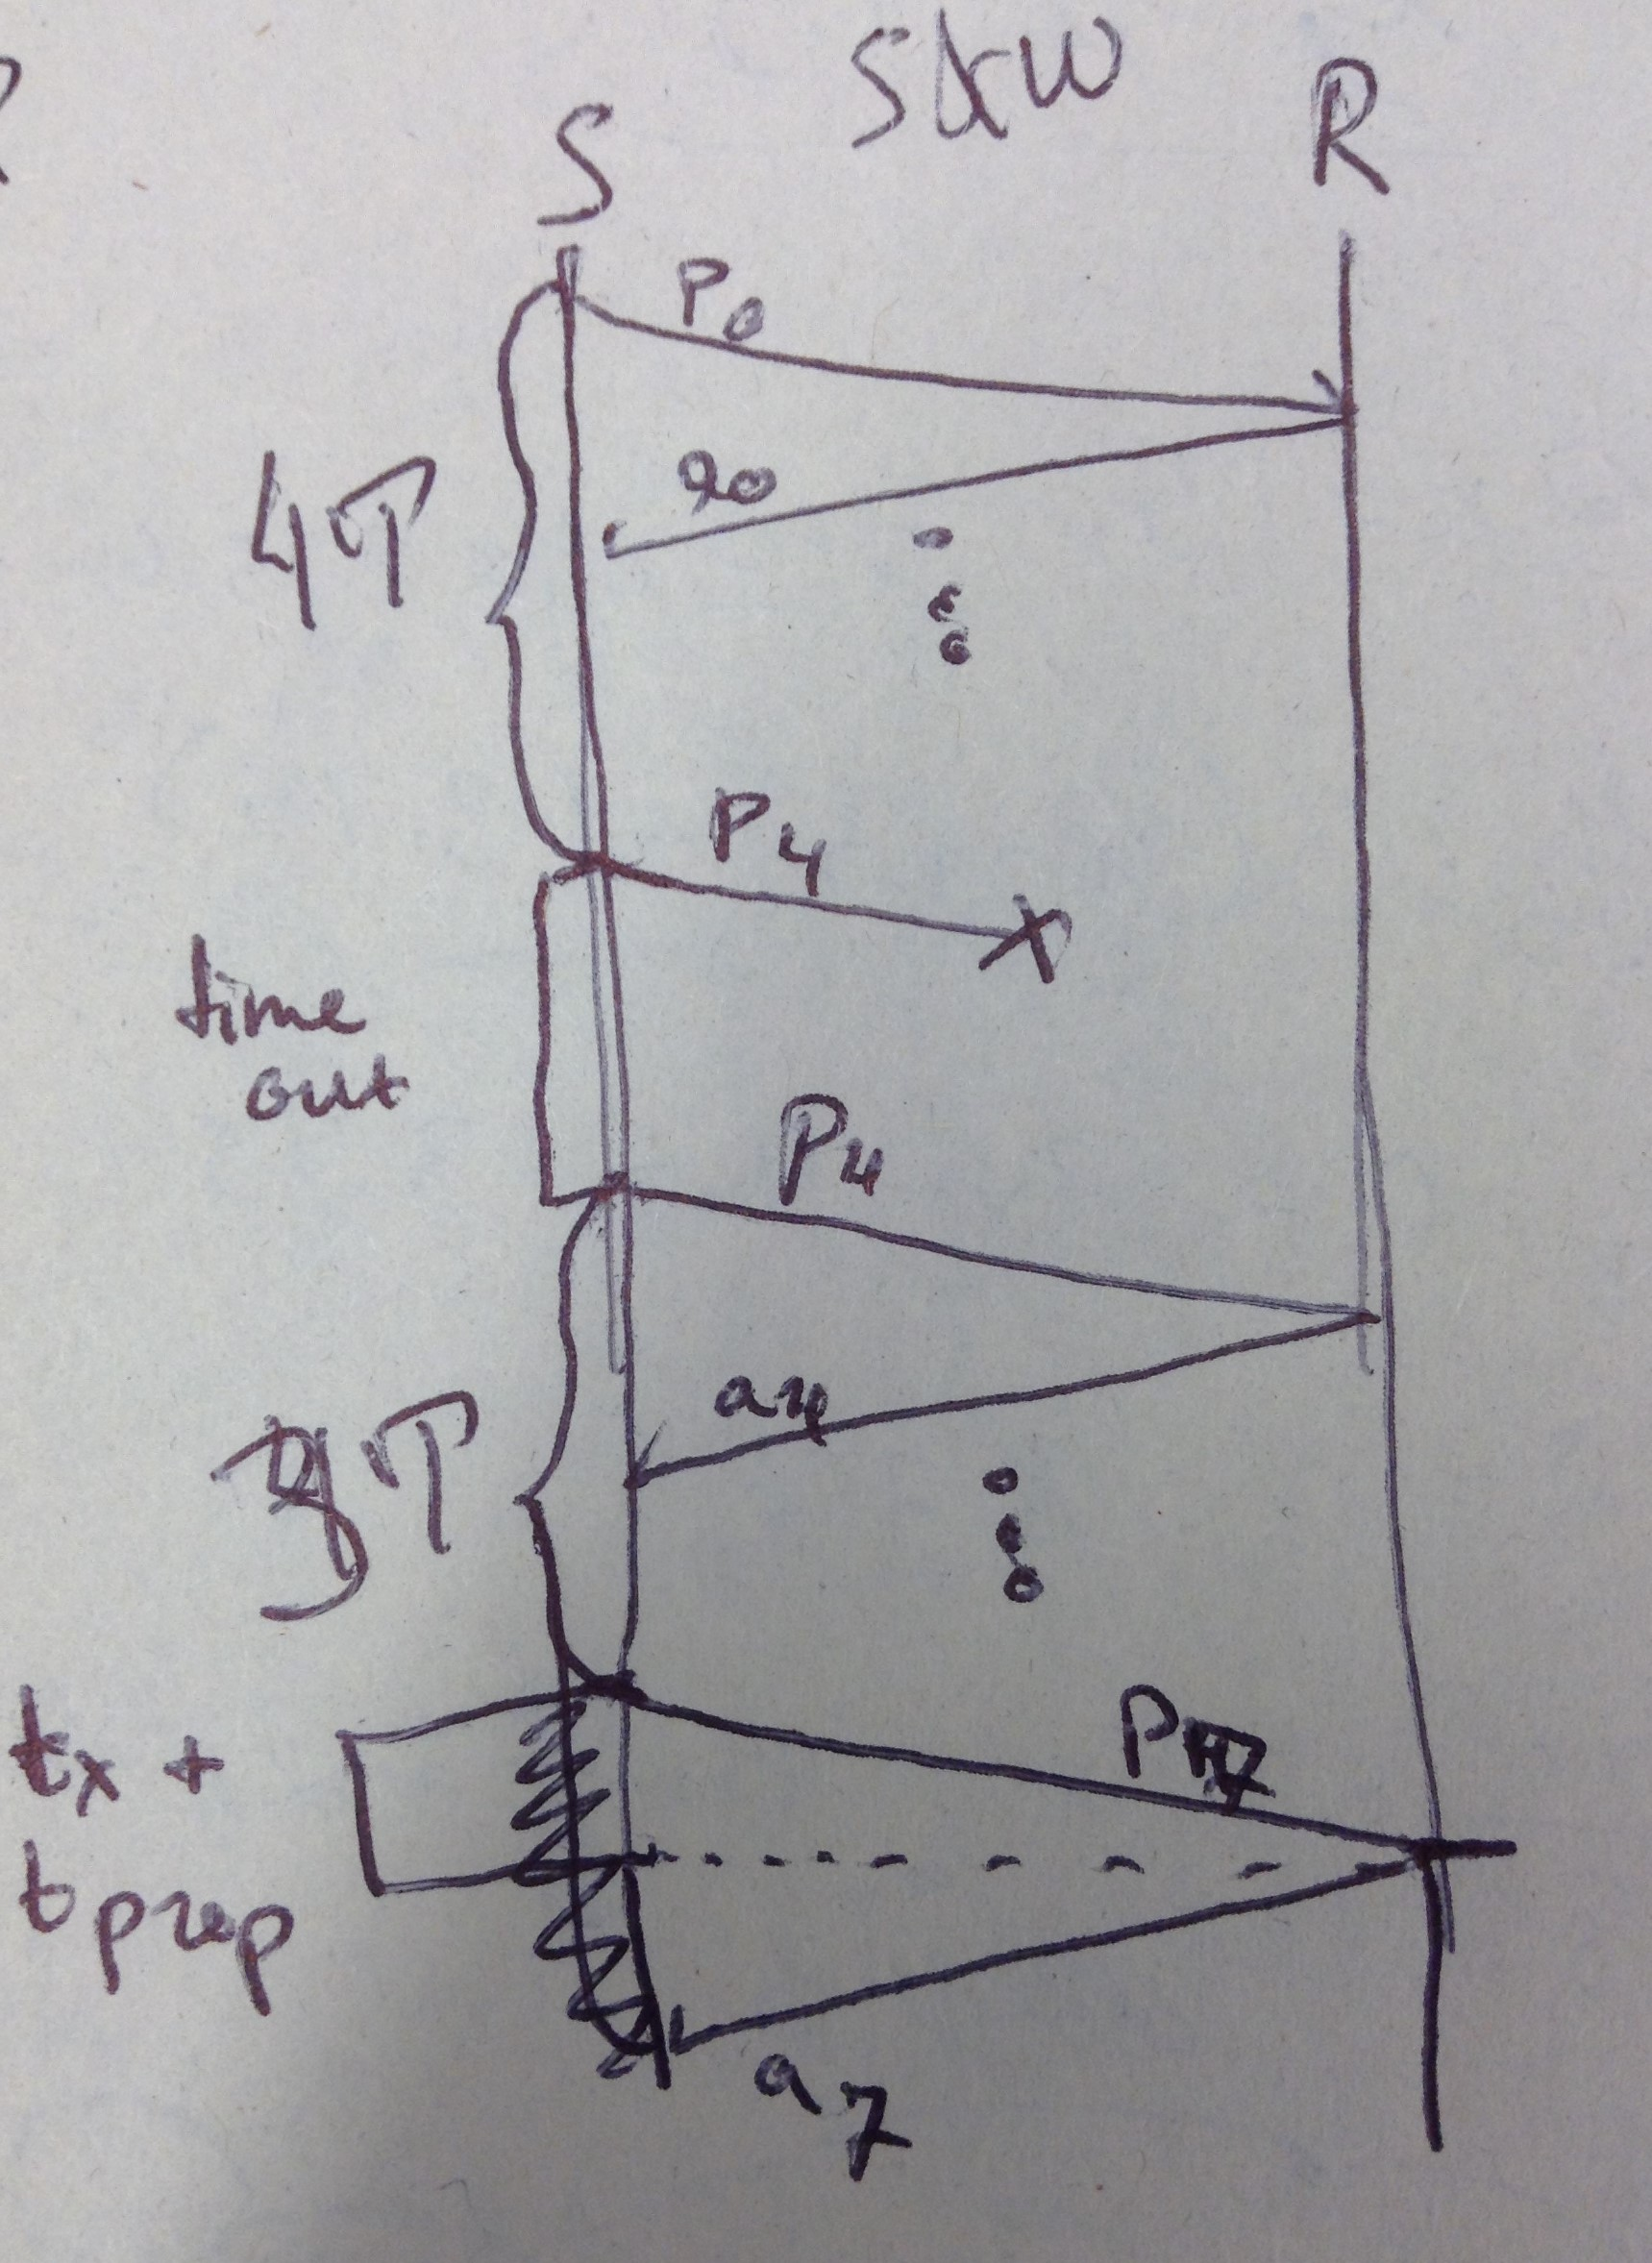
\includegraphics[scale=0.1]{SW_loss}	
				\end{figure}
			\item For GBN, after the fifth packet is sent, the timeout timer starts, after 5 ms, all the packets in the window, which will be packets 5,6,7,\& 8, will be send the receiver. So, $t_{total} = T + 5ms + 4t_{xmit} + t_{prop} = 13ms$.
				\begin{figure}[H]
					\centering
					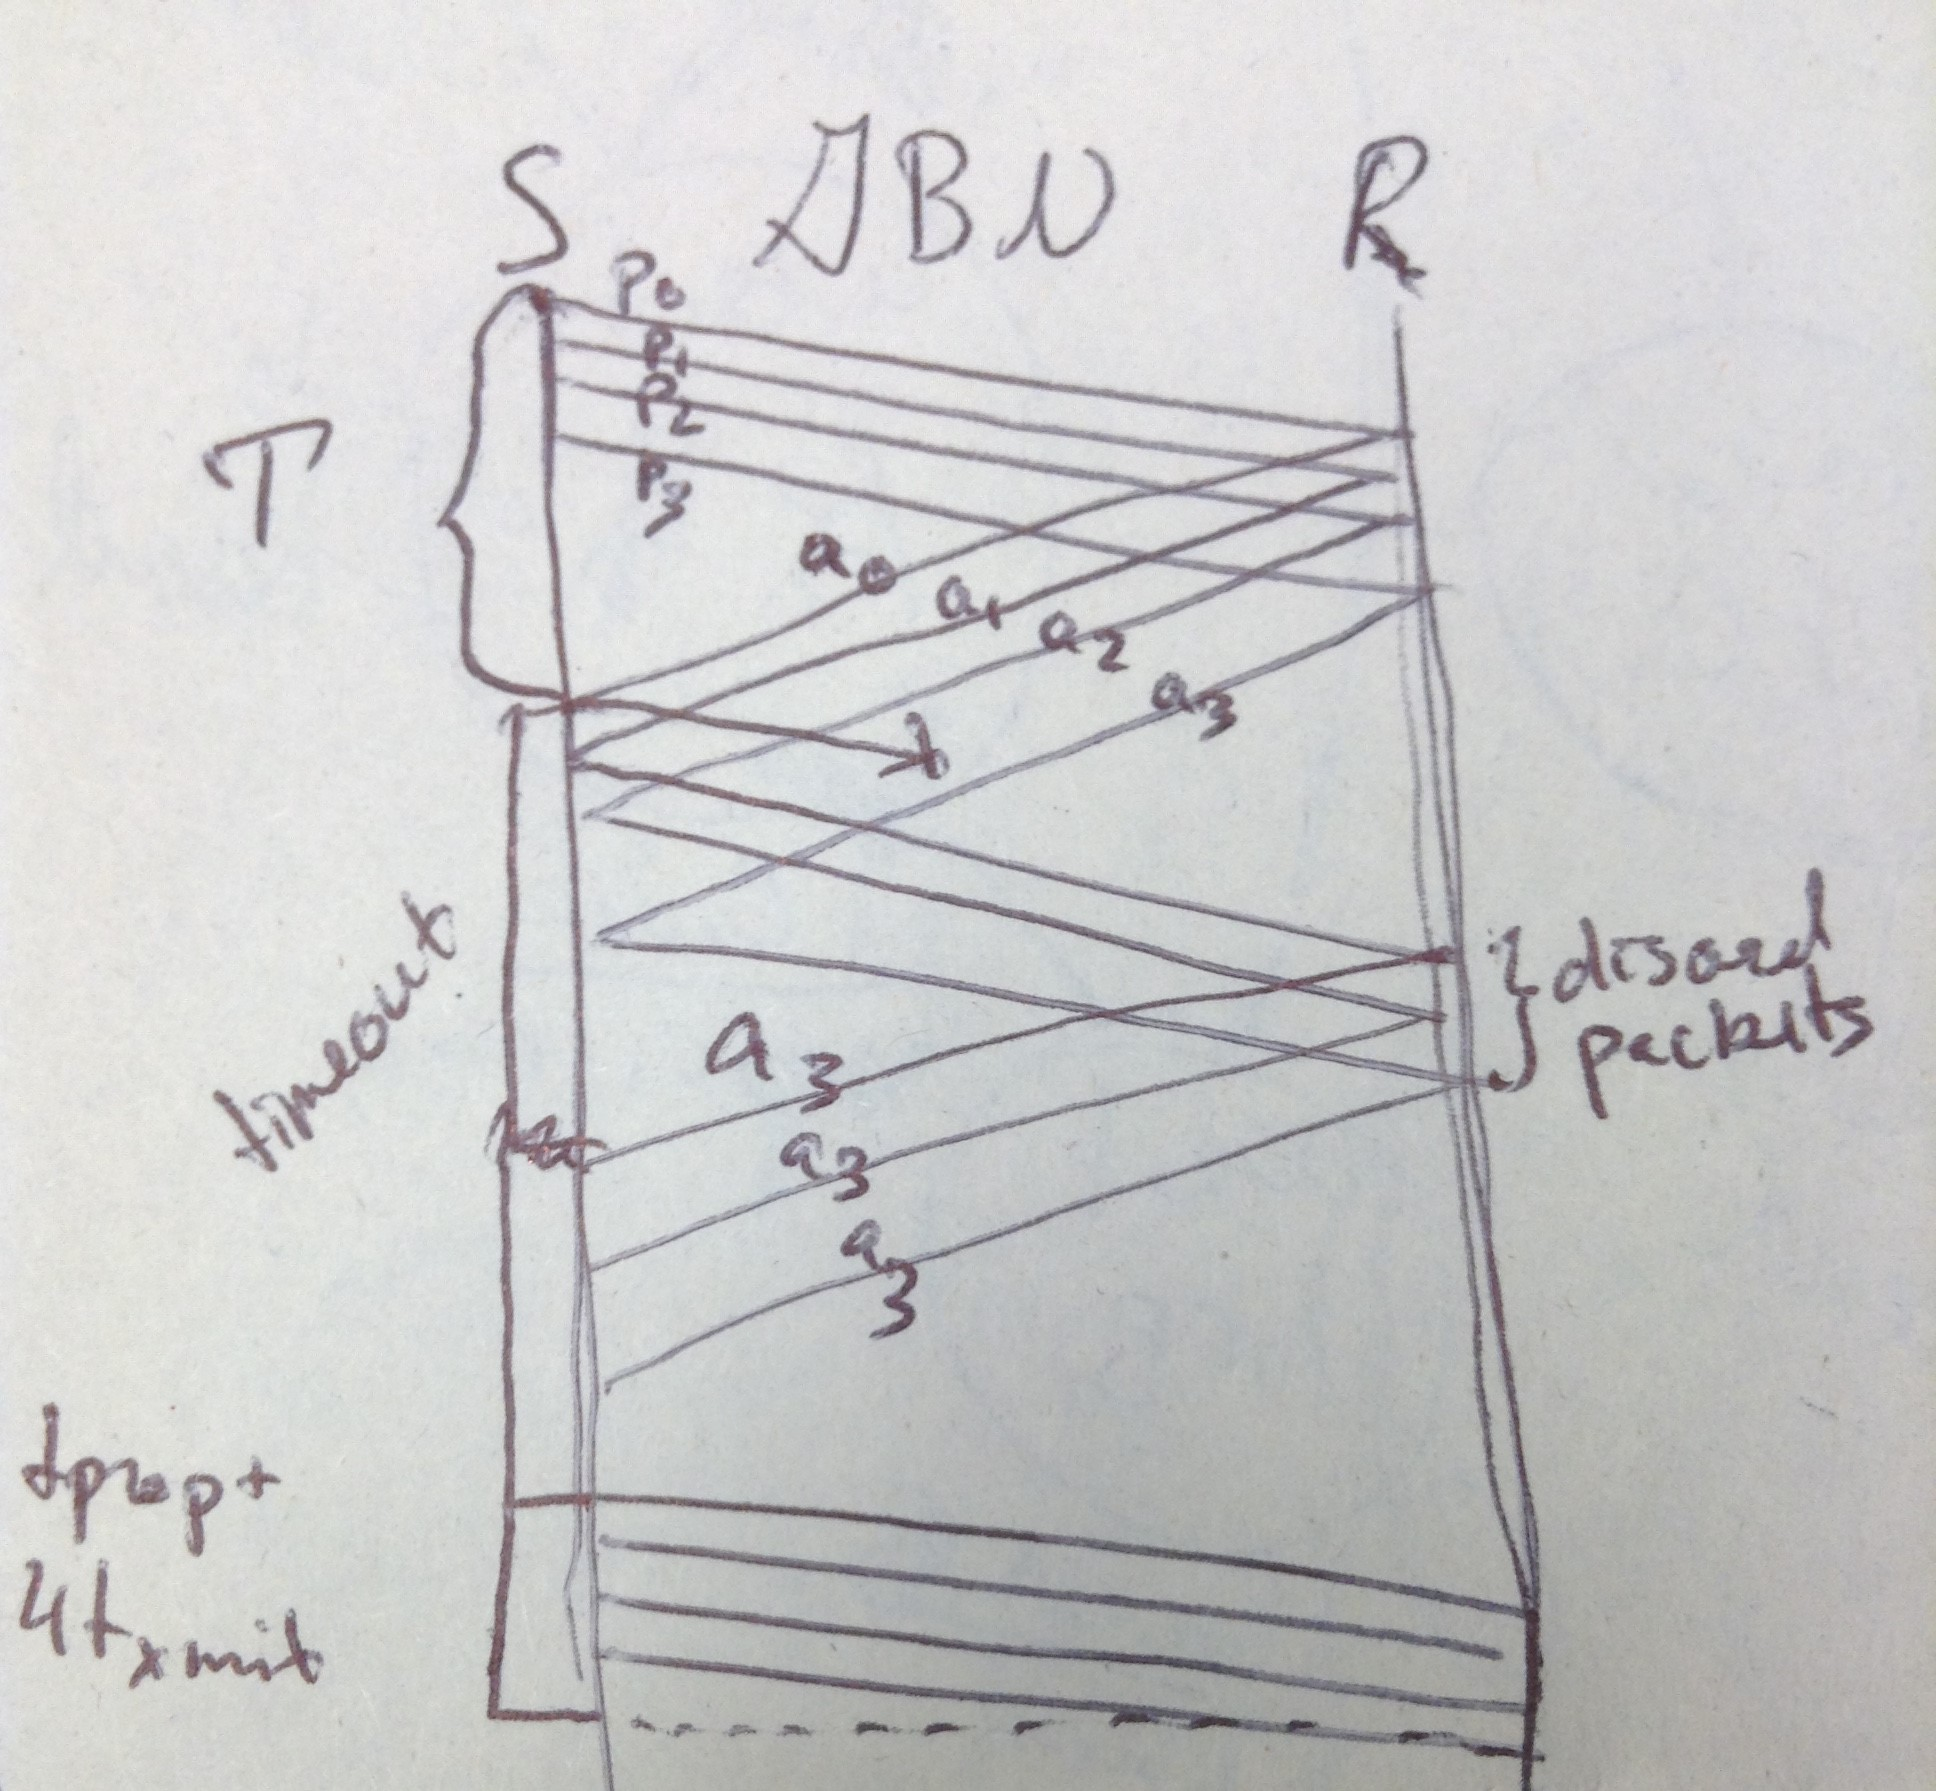
\includegraphics[scale=0.1]{GBN_loss}	
				\end{figure}
			\item In the case of SR, because the receiver can buffer out of order packets and the packets that come acter 5 arrive before the fifth packet times out, the total time is simple the sum of T, the timeout length, and the packet delay. So, $t_{total} = 9ms$.
				\begin{figure}[H]
					\centering
					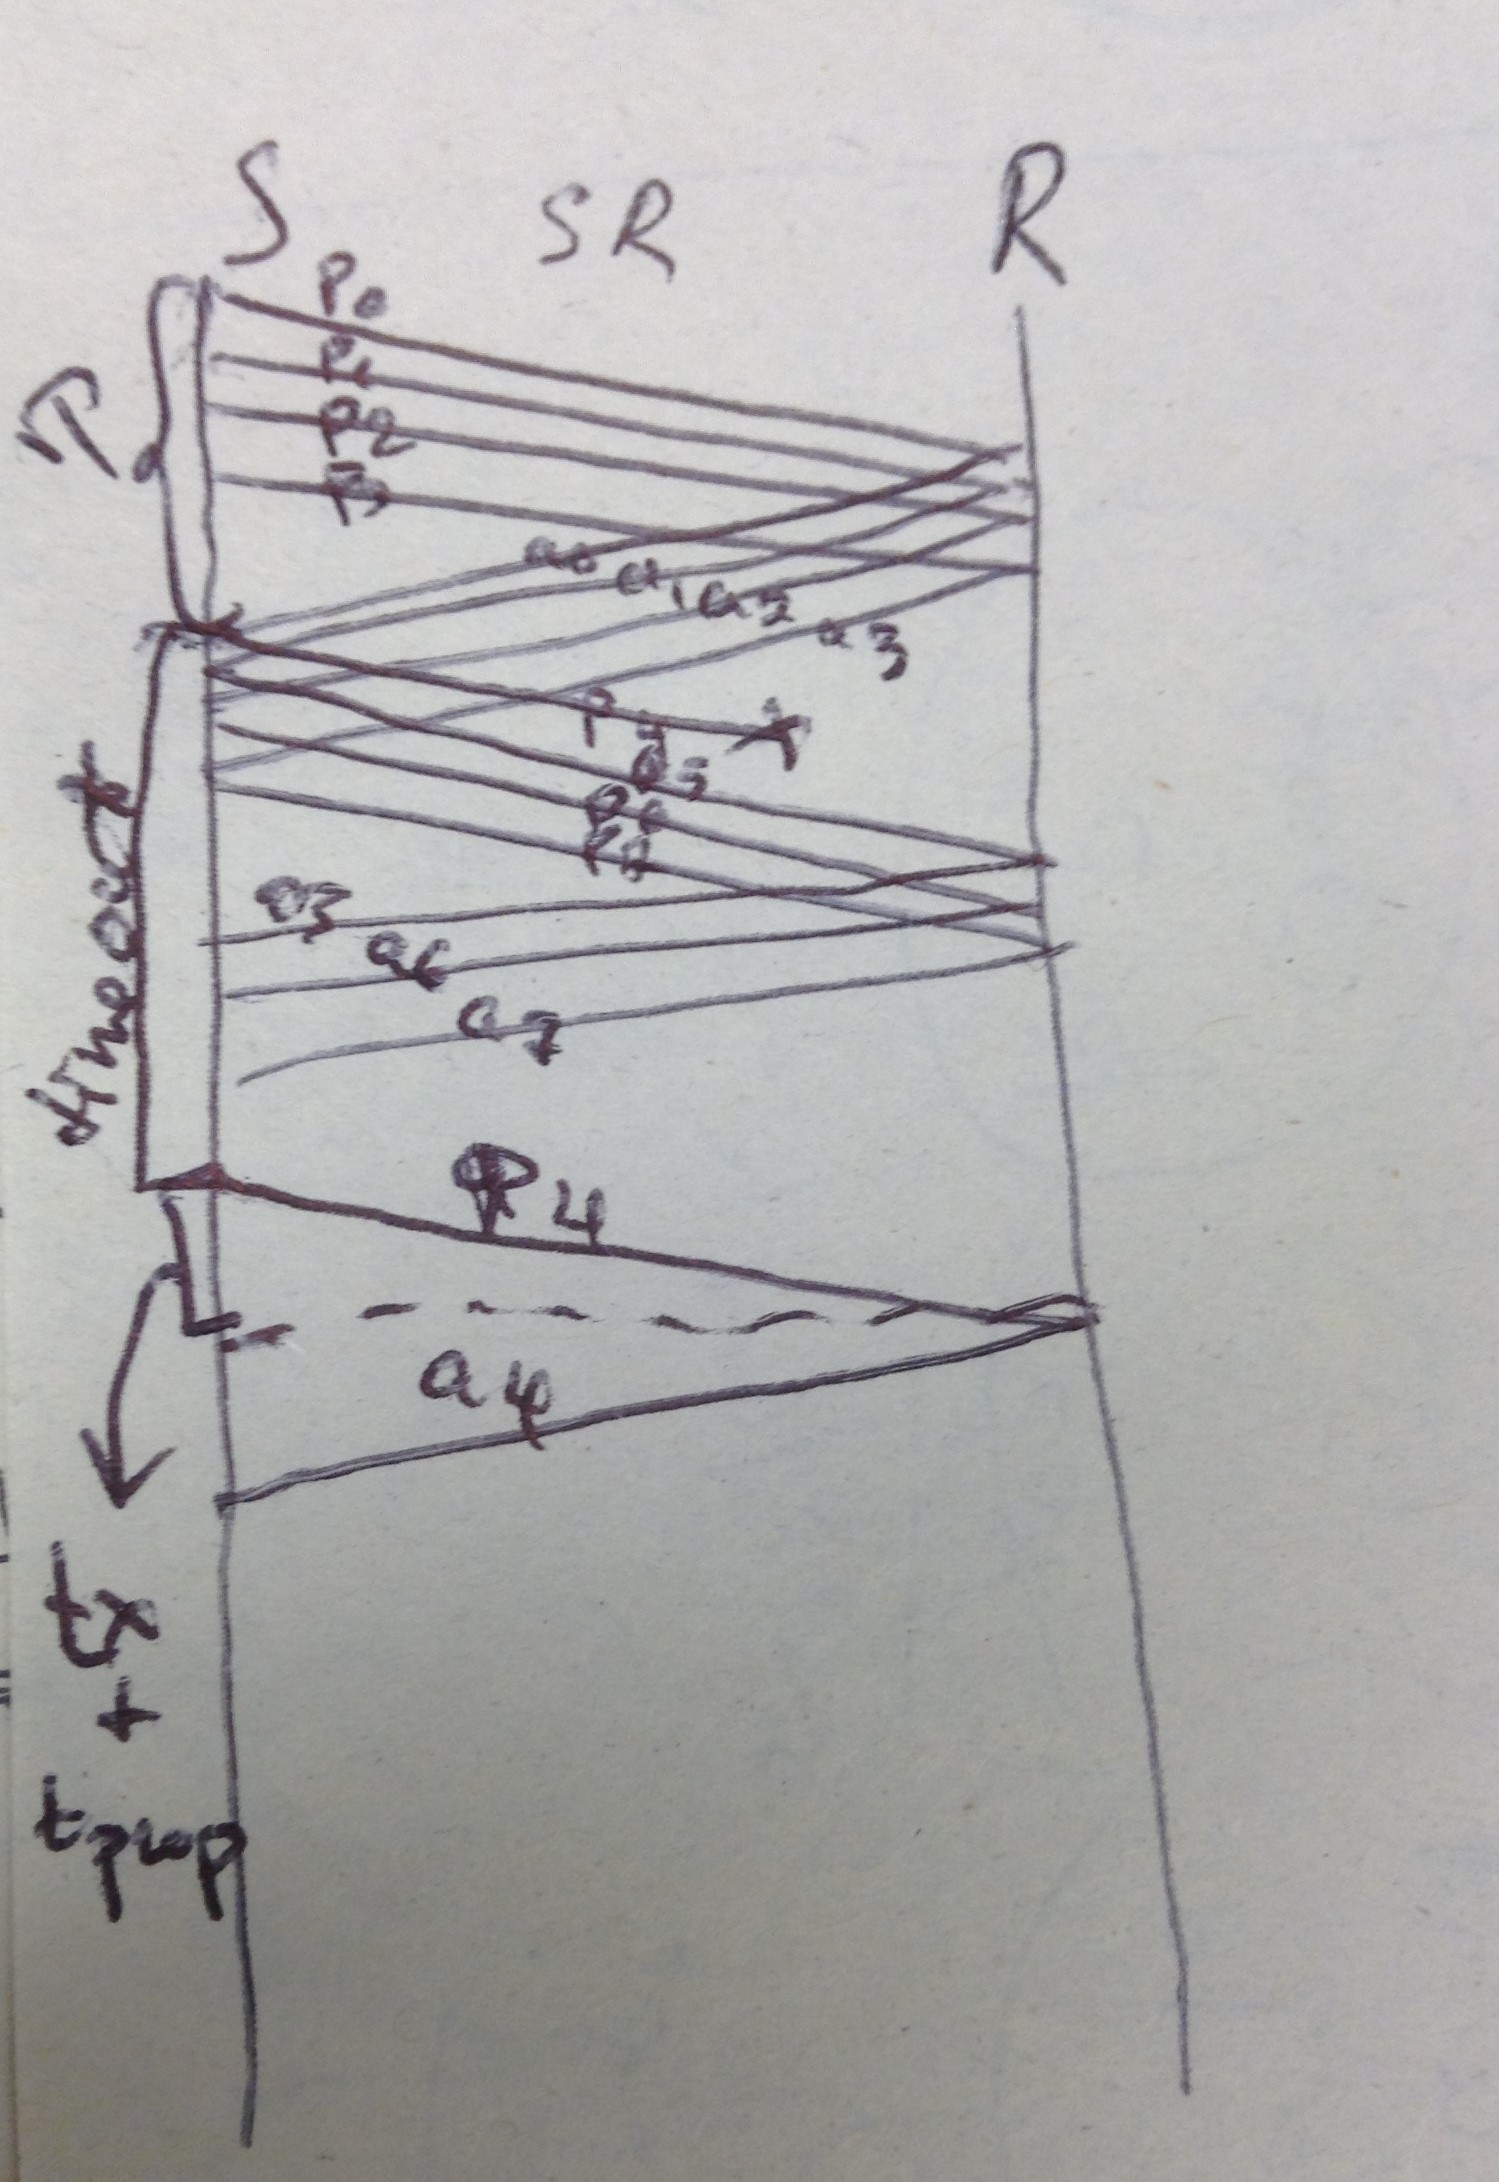
\includegraphics[scale=0.1]{SR_loss}	
				\end{figure}
		\end{enumerate}
\end{enumerate}


\paragraph{Additonal Question 2}
\begin{enumerate}[label=\textbf{Part \alph*)},leftmargin=*,align=left]
	\item The optimal time out would be the expected time for a packet's acknowledgement to be received, which is $2t_{prop} + t_{xmit}$.
	\item Let link utilization be denoted by $U = \frac{t_{xmit}}{2t_{prop} + t_{xmit}}$. If $a = \frac{t_{prop}}{t_{xmit}}$, then $U = \frac{1}{1 + 2a}$. 
		\begin{tabular}{ | l | l | }
			\hline
			a & U(a) \\ \hline
			0.3 &  0.625 \\ \hline
			1    &  0.333 \\ \hline
			3    &  0.143	\\ \hline
		\end{tabular}
	\item Let $\mathcal{E}$ be the event that a packet and/or its acknowledgement is lost. $\mathcal{E}^C$ is then the event that both the packet \& its ack arrive successfully. Then,
		\begin{align*}
			P & = P (\mathcal{E}) \\
			& = 1 - P( \mathcal{E}^C) \\
			& = 1 - (1 - p_{loss})( 1 - p_{loss} ) \\
			& = 1 - ( 1 - 2p_{loss} + p_{loss}^2 ) \\
			& = 2p_{loss} - p_{loss}^2\\
		\end{align*}
	\item Let $\bar{U}$ denot ethe average utilization given by $\bar{U} = \frac{t_{xmit}}{\bar{N}T}$, where T is the time from when the sender sends packt to when it receive that packet's acknowledgement, equal to $t_{xmit} + 2t_{prop}$. $\bar{N} = E[N]$, is the expected value of N, the random binomial variable with probability$1 - p_{loss}$ representing the number of attempts required to send a packet successfully. Thus, $\bar{N} = \frac{1}{1-p_{loss}}$. So then,
		\begin{align*}
			\bar{U} & = \frac{t_xmit}{\frac{ 1 }{ (1 - p_{loss})T } } \\
				       & = \frac{ ( 1 - p_{loss})t_{xmit} }{ T } \\
				       & = ( 1 - p_{loss} )\frac{ 1 }{ 1 + 2a } \\
			\bar{U} & = \frac{ 1 - p_{loss} }{ 1 + 2a } \\
		\end{align*}
		\begin{tabular}{| l | l | l |  }
			\hline
			$P_{loss}$ & a & U(a, $P_loss$ ) \\ \hline
			0.2 & 0.3 & 0.5 \\ \hline
			      & 1.0 & 0.266 \\ \hline
			      & 3.0 & 0.114 \\ \hline
			0.4 & 0.3 & 0.375 \\ \hline
			      & 1.0 & 0.200 \\ \hline
			      & 3.0 & 0.086 \\ \hline
		\end{tabular}
\end{enumerate}
\end{document}
This is never printed